\section{文档类型定义DTD}


\begin{frame}[fragile]{CH3 DTD}
\begin{figure}
    
\includegraphics[width=0.5\textwidth]{figure/dtd.png}
\end{figure}
\end{frame}

\begin{frame}[fragile]{本章学习目标}
\begin{easylist} \easyitem
& 了解 DTD 的作用
& 掌握 DTD 的语法规则和使用方法
& 能够利用 XML 编辑工具实现 DTD 的编辑和验证
\end{easylist}
\end{frame}

\begin{frame}[fragile, allowframebreaks]{目录}
\begin{easylist} \easyitem
& DTD的作用
& DTD的关联方式
&& 内部DTD、外部DTD、公用DTD、内外结合方式
& DTD元素
&& 元素类型声明
&& 空元素
&& 文本类型元素
&& 元素内容模型与混合内容元素
& DTD属性
&& 属性声明
&& 属性类型
&& 属性的默认形态
&& 特殊属性
& DTD实体
&& 实体类型与实体引用
&& 内部可解析通用实体
&& 外部可解析通用实体
&& 外部非解析通用实体
&& 内部参数实体
&& 外部参数实体
& DTD NOTATION
& DTD的包含与忽略
\end{easylist}
\end{frame}

\subsection{3.1 DTD的作用}

\begin{frame}{3.1 DTD的作用}
\par 老师请每一个同学把最近一年看过的5本书写出来,并进行汇总统计,供大家交流学习,要求大家采用XML进行表示,图书信息暂时只包含作者和书名。由于XML表示方式非常自由,不同同学的表示结果很可能不同。
\end{frame}

\begin{frame}[fragile]{第1个同学的XML文档}
\begin{lstlisting}[tabsize=8, basicstyle=\small\tt, language=XML]
<?xml version="1.0"?>
<book>
    <name author="罗贯中">三国演义</name>
    <name author="曹雪芹">红楼梦</name>
    <name author="施耐庵">水浒传</name>
    <name author="吴承恩">西游记</name>
    <name author="荷马">荷马史诗</name>
</book>
\end{lstlisting}
\end{frame}

\begin{frame}[fragile]{第2个同学的XML文档}
\begin{lstlisting}[tabsize=8, basicstyle=\small\tt, language=XML]
<?xml version="1.0"?>
<books>    
    <book title="神曲" author="但丁"/>
    <book title="哈姆雷特" author="莎士比亚"/>
    <book title="浮士德" author="歌德"/>
    <book title="哈克贝利芬历险记" author="马克.吐温"/>
    <book title="少年维特之烦恼" author="歌德"/>
</books>
\end{lstlisting}
\end{frame}

\begin{frame}[fragile]{问题}
\begin{easylist} \easyitem    
& 不同同学所采用的描述方式却不尽相同,这使得后续的自动汇总处理难以实现
& 在实际应用中,“格式良好”仅是一个基本要求,还需要满足一些额外的约束
& DTD通过独特的语法,规定了XML文档编写应遵守的约束
& DTD示例:
\end{easylist}
\begin{lstlisting}[tabsize=8, basicstyle=\small\tt, language=XML]
<!ELEMENT books (book)+>
<!ELEMENT book EMPTY>
<!ATTLIST book 
    title CDATA #REQUIRED
    author CDATA #REQUIRED
>
\end{lstlisting}
\end{frame}



\subsection{3.2 DTD的关联方式}
\begin{frame}[fragile]{3.2 DTD的关联方式}
\begin{easylist} \easyitem    
& 内部DTD
& 外部DTD
& 公用DTD
& 内外结合关联方式
\end{easylist}
\end{frame}

\begin{frame}[fragile]{内部关联方式}
\begin{lstlisting}[tabsize=8, basicstyle=\small\tt, language=XML]
<?xml version="1.0"?>
<!DOCTYPE books [
    <!ELEMENT books (book)+>
    <!ELEMENT book EMPTY>
    <!ATTLIST book 
        title CDATA #REQUIRED
        author CDATA #REQUIRED
    >
]>
<books>    
    <book title="神曲" author="但丁"/>
    <book title="哈姆雷特" author="莎士比亚"/>
    <book title="浮士德" author="歌德"/>
    <book title="哈克贝利芬历险记" author="马克.吐温"/>
    <book title="少年维特之烦恼" author="歌德"/>
</books>
\end{lstlisting}
\end{frame}


\begin{frame}[fragile]{外部关联方式}
\begin{easylist} 
& 当对结构相同的多个XML文档进行验证时,使用外部DTD是最为合适的选择方案
& 既可以使DTD在多个文档中得到复用,方便维护管理,也有利于数据的传输。
\end{easylist}
\end{frame}


\begin{frame}[fragile]{XML文档}
\begin{lstlisting}[tabsize=8, basicstyle=\small\tt, language=XML]
<?xml version="1.0"?>
<!DOCTYPE books SYSTEM "3-2.dtd">
<books>
    <book title="神曲" author="但丁"/>
    <book title="哈姆雷特" author="莎士比亚"/>
    <book title="浮士德" author="歌德"/>
    <book title="哈克贝利芬历险记" author="马克吐温"/>
    <book title="少年维特之烦恼" author="歌德"/>
</books>
\end{lstlisting}
\end{frame}


\begin{frame}[fragile]{DTD文档}
\begin{lstlisting}[tabsize=8, basicstyle=\small\tt, language=XML]
<?xml version="1.0" encoding="UTF-8"?>
<!ELEMENT books (book)+>
<!ELEMENT book EMPTY>
<!ATTLIST book 
    title CDATA #REQUIRED
    author CDATA #REQUIRED
>
\end{lstlisting}
\end{frame}


\begin{frame}[fragile]{公用DTD}
\begin{easylist} 
& 关键字SYSTEM并非关联外部DTD文档的唯一方式, SYSTEM关键字适用于在私有组织内部或个人多个文档之间对DTD的共享使用。使用PUBLIC关键字的公用DTD是另一种常见的关联方式
& XML文档与公用DTD的关联方式
&& <!DOCTYPE 根元素名称 PUBLIC FPI "DTD\_URL">
&& FPI: Formal Public Identifier,规范化公共标识符
\end{easylist}
\end{frame}


\begin{frame}[fragile]{FPI}
\begin{shaded}
\par 初始化字符串//DTD所有者名称//DTD描述//语言标识符
\end{shaded}
\begin{easylist} 
& 初始化字符串
&& 如果DTD是一个ISO标准,则DTD名称以字符串“ISO”开始;
&& 如果DTD由某个非ISO组织所同意,那么名称以“+”开始;
&& 如果没有标准化组织同意该DTD,则名称以“-”开始。
& 例子
\end{easylist}

\begin{lstlisting}[tabsize=8, basicstyle=\small\tt, language=XML]
<!DOCTYPE html PUBLIC "-//W3C//DTD XHTML 1.0 Transitional//EN" 
"http://www.w3.org/TR/xhtml1/DTD/xhtml1-transitional.dtd">

<!DOCTYPE CONTACTS PUBLIC "-//xiatian//Contact Data//EN"
                "http://www.mydomain.com/dtds/contacts.dtd">
\end{lstlisting}
\end{frame}


\begin{frame}[fragile]{内外结合方式}
\begin{easylist} 
& 内部DTD和外部DTD合并使用
\end{easylist}
\end{frame}

\begin{frame}[fragile]{E.g. 外部DTD}
\begin{lstlisting}[tabsize=8, basicstyle=\small\tt, language=XML]
<?xml version="1.0" encoding="UTF-8"?>
<!ELEMENT universities (university)+>
<!ELEMENT university (#PCDATA)>
<!ENTITY RUC "中国人民大学">
\end{lstlisting}
\end{frame}

\begin{frame}[fragile]{E.g. XML文档}
\begin{lstlisting}[tabsize=8, basicstyle=\small\tt, language=XML]
<?xml version="1.0"?>
<!DOCTYPE universities SYSTEM "3-5.dtd"[
    <!ENTITY RUC "人民大学">
]>
<universities>    
    <university>&RUC;</university>
    <university>北京大学</university>
    <university>清华大学</university>
</universities>
\end{lstlisting}

\begin{easylist} 
& 同时使用了外部DTD和内部DTD定义方式
& 内部DTD会覆盖外部DTD已有定义
\end{easylist}
\end{frame}



\subsection{3.3 DTD元素}
\begin{frame}[fragile]{3.3 DTD元素}
\begin{easylist} \easyitem    
& 元素类型声明
& 空元素
& 文本类型元素
& 元素内容模型与混合内容元素
\end{easylist}
\end{frame}


\subsubsection{3.3.1 元素类型声明}
\begin{frame}[fragile]{3.3.1 元素类型声明}
\begin{shaded}
\par 语法:<!ELEMENT 元素名称 元素内容规范>
\end{shaded}

\begin{easylist} \easyitem    
& ELEMENT作为关键字,用于对指定元素进行声明
& ELEMENT单词必须全部大写
& ELEMENT与“<!”之间不能留有空格
& 元素内容规范指明了元素内可以包含的内容形式
&& 空元素(EMPTY)
&& 任意元素(ANY)
&& 父元素
&& 文本元素
&& 混合元素
\end{easylist}
\end{frame}


\begin{frame}[fragile]{Example}
\begin{lstlisting}[tabsize=8, basicstyle=\small\tt, language=XML]
<?xml version="1.0" encoding="UTF-8"?>
<!ELEMENT books ANY>
<!ELEMENT book (title, author, publish)>
<!ELEMENT title (#PCDATA)>
<!ELEMENT author (#PCDATA)>
<!ELEMENT publish (#PCDATA|ISBN)*>
<!ELEMENT ISBN EMPTY>
\end{lstlisting}
\end{frame}


\subsubsection{3.3.2 空元素}
\begin{frame}[fragile]{3.3.2 空元素}
\begin{easylist} \easyitem
& 语法
\begin{lstlisting}[tabsize=8, basicstyle=\small\tt, language=XML, numbers=none]
<!ELEMENT 元素名 EMPTY>
\end{lstlisting}
& 例子
\begin{lstlisting}[tabsize=8, basicstyle=\small\tt, language=XML]
<!ELEMENT 人物 EMPTY>
<!ELEMENT IMG EMPTY>
\end{lstlisting}

& 使用场景
&& 元素把全部数据放在属性里,而元素本身没有任何PCDATA内容
&& 例如:
\begin{lstlisting}[tabsize=8, basicstyle=\small\tt, language=XML]
<人物 姓名="林冲" 籍贯="东京" 职业="强盗" 特长="枪棒"/>
<img src="baby.jpg" alt="baby" title="宝贝的照片"/>
\end{lstlisting}
\end{easylist}
\end{frame}


\subsubsection{3.3.3 文本类型元素}
\begin{frame}[fragile]{3.3.3 文本类型元素}
\begin{easylist} \easyitem    
& 语法:
\begin{lstlisting}[tabsize=8, basicstyle=\small\tt, language=XML]
<!ELEMENT 元素名 (#PCDATA) >
\end{lstlisting}

& 例子
\begin{lstlisting}[tabsize=8, basicstyle=\small\tt, language=XML]
<!ELEMENT 姓名 (#PCDATA)>
<!ELEMENT 籍贯 (#PCDATA)>
\end{lstlisting}

&& \#PCDATA为元素数据的指定类型
&&& Parsed Character Data:可解析字符数据
&&& 元素把全部数据放在属性里,本身没有任何PCDATA内容

& DTD类型限制
&& 不能区分文本和数字,无法区分整数和实数
&& 不能定义用户数据类型
&& 不能限制数据的取值范围
\end{easylist}
\end{frame}


\begin{frame}[fragile]{以下定义方式是否正确?}
\begin{lstlisting}[tabsize=8, basicstyle=\small\tt, language=XML]
<!ELEMENT 姓名 #PCDATA>
<!ELEMENT 姓名 PCDATA>
\end{lstlisting}

\end{frame}


\subsubsection{3.3.4 元素内容模型与混合内容元素}
\begin{frame}[fragile]{3.3.4 元素内容模型与混合内容元素}
\begin{shaded}
\par 元素内容模型ECM(Element Content Models)就是用来描述元素内具体可以包含哪些子元素的一组正则表达式
\end{shaded}
\begin{table}[!hbp] 
\begin{tabular}{|c|c|c|}
\Xhline{1.3pt}
元字符 & 用法 & 范例 \\
\Xhline{1.3pt}
, & 将各个元素依指定顺序排列 & (A,B,C) \\
\hline
字符串 &  一个元素仅能出现一次 &  (A) \\
\hline
* & 元素可以出现0次或0次以上 & A*\\
\hline
+ & 元素可以出现1次或1次以上 & A+\\
\hline
? & 一个元素可以出现0次或一次 & A? \\
\hline
( ) & 分组符号,常结合“,”或“|”使用 &  (A,B) \\
\hline
|  &  逻辑或,只能出现符号作用范围的任一元素1次 & (A|B|C)\\
\hline
\end{tabular}
\caption{元素内容模型的元字符以及相应用法与范例}
\end{table}
\end{frame}


\begin{frame}[fragile]{具有严格顺序的子元素序列}
\begin{shaded}
对内容规范为逗号分隔的子元素序列,文档必须严格按照规定的顺序来书写子元素
\end{shaded}

\begin{lstlisting}[tabsize=8, basicstyle=\small\tt, language=XML]
<?xml version="1.0" encoding="UTF-8" standalone="yes"?>
<!DOCTYPE person [
    <!ELEMENT person (name, telephone, email)>
    <!ELEMENT name (#PCDATA)>
    <!ELEMENT email (#PCDATA)>
    <!ELEMENT telephone (#PCDATA)>    
]>
<person>
    <name>Summer</name>
    <email>summer@ruc.edu.cn</email>
    <telephone>010-82500673</telephone>    
</person>
\end{lstlisting}
\begin{easylist} \easyitem    
& 思考以上XML是否有效?
\end{easylist}
\end{frame}


\begin{frame}[fragile]{可重复元素}
\begin{easylist} \easyitem    
& 若某子元素名后跟有星号“*”或加号“+”,则该元素可以重复若干次
& +代表出现1到多次,即至少出现一次
& *代表出现0到多次,即可以不出现
\end{easylist}

\begin{lstlisting}[tabsize=8, basicstyle=\small\tt, language=XML]
<?xml version="1.0" encoding="UTF-8" standalone="yes"?>
<!DOCTYPE person [
    <!ELEMENT person (name, telephone, email+)>
    <!ELEMENT name (#PCDATA)>
    <!ELEMENT email (#PCDATA)>
    <!ELEMENT telephone (#PCDATA)>    
]>
<person>
    <name>Summer</name>
    <telephone>010-82500673</telephone>    
    <email>summer@ruc.edu.cn</email>
    <email>xia@ruc.edu.cn</email>
</person>
\end{lstlisting}
\end{frame}


\begin{frame}[fragile]{分组与逻辑或}
\begin{easylist} \easyitem    
& 逻辑或“|”用于多选一情况,经常与分组符号“( )”结合使用
& Eaxmple:
\begin{lstlisting}[tabsize=8, basicstyle=\small\tt, language=XML, numbers=none]
<!ELEMENT person (name, (telephone | email) )>
\end{lstlisting}

&& 元素person的子元素name后面只能有一个telephone元素或者email元素,而不能两个都有。
&& 错误写法: 
\begin{lstlisting}[tabsize=8, basicstyle=\small\tt, language=XML, numbers=none]
<!ELEMENT person (name, telephone | email )>
\end{lstlisting}

& 以下DTD语句的含义是什么?
\begin{lstlisting}[tabsize=8, basicstyle=\small\tt, language=XML, numbers=none]
 <!ELEMENT person (name, (telephone | email | (telephone, email) ) )>
\end{lstlisting}

\end{easylist}
\end{frame}


\begin{frame}[fragile]{可选元素}
\begin{easylist} \easyitem    
& 子元素后面跟有问号符号“?”,属于可选元素,可以出现0次或1次
& 当无法确定一个元素是否会出现而且就算出现也只出现一次,可以使用该符号
& E.g. 
\begin{lstlisting}[tabsize=8, basicstyle=\small\tt, language=XML, numbers=none]
<!ELEMENT person (name, (areaCode?, telephone), email )>
\end{lstlisting}
&& person元素中的联系电话部分必须出现telephone子元素,而区号areaCode,则可以出现,也可以不出现
\end{easylist}
\end{frame}


\begin{frame}[fragile]{混合内容}
\begin{easylist} \easyitem    
& 假设采用XML对人物信息进行描述,描述内容采用文本形式,但同时希望文本内出现的人物姓名、籍贯、职业等信息采用元素方式进行结构化表示,也就是说,子元素可以任意散布在一段段的文本之中。
& 可采用混合内容描述方法:
\begin{lstlisting}[tabsize=8, basicstyle=\small\tt, language=XML, numbers=none]
<!ELEMENT 元素名 (#PCDATA | 子元素1 | 子元素2 | … | 子元素n)* >
\end{lstlisting}
\end{easylist}
\end{frame}


\begin{frame}[fragile]{混合内容示例}
\begin{lstlisting}[tabsize=8, basicstyle=\small\tt, language=XML]
<?xml version="1.0" encoding="UTF-8" standalone="yes"?>
<!DOCTYPE 人物 [
    <!ELEMENT 人物 (#PCDATA|姓名|籍贯|职业|特长)* >
    <!ELEMENT 姓名 (#PCDATA)>
    <!ELEMENT 籍贯 (#PCDATA)>
    <!ELEMENT 职业 (#PCDATA)>
    <!ELEMENT 特长 (#PCDATA)>
]>
<人物>
    <姓名>林冲</姓名>,<籍贯>东京</籍贯>人氏,人称豹子头,
官方认定其为水泊梁山<职业>强盗</职业>。
生性耿直,爱交好汉,擅长<特长>枪棒</特长>。
</人物>
\end{lstlisting}

\begin{easylist} \easyitem    
& <!ELEMENT 人物 (\#PCDATA|姓名|籍贯|职业|特长)* >
\end{easylist}
\end{frame}



\subsection{3.4 DTD属性}
\begin{frame}[fragile]{3.4 DTD属性}
\begin{easylist} \easyitem    
& 属性声明
& 属性类型
& 属性的默认形态
& 特殊属性
\end{easylist}
\end{frame}


\subsubsection{3.4.1 属性声明}
\begin{frame}[fragile]{3.4.1 属性声明}
\begin{easylist} \easyitem    
& 语法:
\begin{lstlisting}[tabsize=8, basicstyle=\small\tt, language=XML, numbers=none]
<!ATTLIST 元素名  属性名  属性类型  缺省声明  (属性名 属性类型 缺省声明… ) >
\end{lstlisting}

&& 元素名指明了属性所属的元素名称
&& 属性名表示指定属性的名称
&& 属性类型决定了属性值应具备的类型,如常用的CDATA
&& 缺省声明规定对属性值的要求和指定默认值
\end{easylist}
\end{frame}


\begin{frame}[fragile]{属性声明示例}
\begin{easylist} \easyitem    
& 如下XML文档片段如何声明对应的DTD?
\begin{lstlisting}[tabsize=8, basicstyle=\small\tt, language=XML, numbers=none]
<人物 姓名="林冲"/>
\end{lstlisting}
\end{easylist}
\end{frame}

\begin{frame}[fragile]{属性声明示例}
\begin{easylist} \easyitem    
& 声明方式:
\begin{lstlisting}[tabsize=8, basicstyle=\small\tt, language=XML]
<!ELEMENT 人物 EMPTY>
<!ATTLIST 人物 姓名 CDATA  #REQUIRED >
\end{lstlisting}

&& <!ELEMENT>标记声明“人物”元素为一个空元素
&& <!ATTLIST>标记表明了“人物”元素拥有属性“姓名”,
&& 人物属性类型为CDATA
&& 人物属性使用时必须指明。
\end{easylist}
\end{frame}



\begin{frame}[fragile]{属性简写方式}
\begin{easylist} \easyitem    
& XML:
\begin{lstlisting}[tabsize=8, basicstyle=\small\tt, language=XML, numbers=none]
<人物 姓名="林冲" 籍贯="东京" 职业="强盗" 特长="枪棒"/>
\end{lstlisting}

& 属性逐个声明方式:
\begin{lstlisting}[tabsize=8, basicstyle=\small\tt, language=XML]
<!ELEMENT 人物 EMPTY>
<!ATTLIST 人物    姓名 CDATA #REQUIRED >
<!ATTLIST 人物    籍贯 CDATA #IMPLIED >
<!ATTLIST 人物    职业 CDATA #IMPLIED >
<!ATTLIST 人物    特长 CDATA "武术" >
\end{lstlisting}

& 属性一起声明方式:
\begin{lstlisting}[tabsize=8, basicstyle=\small\tt, language=XML]
<!ATTLIST 人物    姓名 CDATA #REQUIRED
                籍贯 CDATA #IMPLIED
                职业 CDATA #IMPLIED
                特长 CDATA "武术">
\end{lstlisting}
\end{easylist}
\end{frame}


\subsubsection{3.4.2 属性类型}
\begin{frame}[fragile]{3.4.2 属性类型}
\begin{table}[!htp] 
\begin{tabular}{|c|l|}
\Xhline{1.3pt}
类型 & 含义 \\
\Xhline{1.3pt}
CDATA & 属性值为任意合法的字符串,最为常用的属性类型 \\ \hline
Enumerated & 从若干个指定值列表中选择正确的值 \\ \hline
ID &  属性值必须唯一,不能与中其他ID类型属性取相同值 \\ \hline
IDREF & 属性值引用了某一个已经指定的ID类型的属性值 \\ \hline
IDREFS & 属性值由多个IDREF类型的属性值组成,并由空格隔开  \\ \hline
NMTOKEN & Name Token,由符合标记命名要求的字符串组成\\ \hline
NMTOKENS & 该属性值是由空格分隔的一系列NMTOKEN的集合 \\ \hline
ENTITY & 属性值为已经由DTD声明的实体名称  \\ \hline
ENTITIES & 属性值是由空格分隔的一系列ENTITY的集合 \\ \hline
NOTATION & 属性值必须匹配NOTATION名称列表中的某个名称 \\     \hline
\end{tabular}
\caption{DTD的属性类型}
\end{table}
\end{frame}


\begin{frame}[fragile]{CDATA属性类型}
\begin{easylist} \easyitem    
& 字符数据(Character DATA),是最基本的属性类型
& 属性值为不包含小于号“<”和“&”的任意文本字符串
& 如出现“<”和“\&”,需要转义
\begin{lstlisting}[tabsize=8, basicstyle=\small\tt, language=XML]
<?xml version="1.0" encoding="UTF-8" standalone="yes"?>
<!DOCTYPE todolist [
    <!ELEMENT todolist (todo)*>
    <!ELEMENT todo EMPTY>
    <!ATTLIST todo content CDATA #REQUIRED> 
]>
<todolist>
    <todo content="当股价>100的时候抛出'全聚德'"/>
    <todo content="周六&amp;周日回山东临朐"/>
</todolist>
\end{lstlisting}
\end{easylist}
\end{frame}


\begin{frame}[fragile]{Enumerated枚举类型}
\begin{easylist} \easyitem    
& 语法:
\begin{lstlisting}[tabsize=8, basicstyle=\small\tt, language=XML, numbers=none]
<!ATTLIST 元素名 属性名 (属性值1 | 属性值2 | … | 属性值n) 缺省声明>
\end{lstlisting}
& 例子:
\begin{lstlisting}[tabsize=8, basicstyle=\small\tt, language=XML, numbers=none]
<!ATTLIST 交易    货币单位 (人民币 | 日元 | 美元 | 欧元 | 英镑)  "人民币">
\end{lstlisting}
\end{easylist}
\end{frame}


\begin{frame}[fragile]{NOTATION符号类型}
\begin{lstlisting}[tabsize=8, basicstyle=\small\tt, language=XML]
<!ELEMENT 图片 (#PCDATA)>
<!NOTATION gif SYSTEM "IMAGE/gif">
<!NOTATION jpg SYSTEM "IMAGE/jpeg">
<!NOTATION png SYSTEM "IMAGE/png">
<!ATTLIST 图片 格式 NOTATION (gif | jpg | png) #REQUIRED>

<图片 格式="png"/>
\end{lstlisting}
\end{frame}


\begin{frame}[fragile]{ID、IDREF与IDREFS属性类型}
\begin{easylist} \easyitem    
& ID: 
&& 该类型的属性无缺省值,缺省声明必须为\#REQUIRED或\#IMPLIED
&& 一个元素不能拥有超过一个ID类型的属性
& IDREF(ID Reference)
&& 对ID的引用,当某个属性引用了另一个ID类型的属性值时,可将其声明为IDREF
& IDREFS(ID References)
&& 多个标识符的引用,属性值引用了多个由空格分隔的ID类型的属性值
\end{easylist}
\end{frame}


\begin{frame}[fragile]{ID、IDREF与IDREFS示例}
\begin{lstlisting}[tabsize=8, basicstyle=\small\tt, language=XML]
<?xml version="1.0" encoding="UTF-8" standalone="yes"?>
<!DOCTYPE 班级 [
    <!ELEMENT 班级 (学生)*>
    <!ELEMENT 学生 (#PCDATA)>    
    <!ATTLIST 班级 名称 CDATA #REQUIRED>
    <!ATTLIST 班级 班长 IDREF #IMPLIED>
    <!ATTLIST 班级 班委 IDREFS #IMPLIED>
    <!ATTLIST 学生 学号 ID #REQUIRED>
]>
<班级 名称="政务信息一班" 班长="S001" 班委="S001 S002 S004">
    <学生 学号="S001">姜海明</学生>
    <学生 学号="S002">李学健</学生>
    <学生 学号="S003">方路</学生>
    <学生 学号="S004">刘杨</学生>
</班级>
\end{lstlisting}
\end{frame}


\begin{frame}[fragile]{NMTOKEN与NMTOKENS属性类型}
\begin{easylist} \easyitem    
& NMTOKEN: Name Token
&& 限定属性值为有效的XML名称
& NMTOKENS: Name Tokens
&& 一组NMTOKEN类型的字符串,每个NMTOKEN之间以空格分隔
\begin{lstlisting}[tabsize=8, basicstyle=\small\tt, language=XML]
<!ELEMENT 数据 (#PCDATA) >
<!ATTLIST 数据    授权用户 NMTOKENS #IMPLIED>

<数据 授权用户="Lucy Summer Macy">如何学好XML的超级技巧……</数据>
\end{lstlisting}
\end{easylist}
\end{frame}


\begin{frame}[fragile]{ENTITY与ENTITIES属性类型}
\begin{easylist} \easyitem    
& ENTITY
&& 限定属性值为已经声明过的实体名称,
& ENTITIES
&& 可以包含多个实体,实体之间通过空格进行分隔。
\end{easylist}
\end{frame}


\begin{frame}[fragile]{ENTITY与ENTITIES示例}
\begin{lstlisting}[tabsize=8, basicstyle=\small\tt, language=XML]
<?xml version="1.0" encoding="UTF-8"?>
<!DOCTYPE 高校列表 [
    <!ELEMENT 高校列表 (高校)*>
    <!ELEMENT 高校 (#PCDATA)>
    <!ATTLIST 高校 LOGO ENTITY #REQUIRED
                   校园风景 ENTITIES #IMPLIED>
    <!NOTATION JPG SYSTEM "image/jpeg">
    <!ENTITY LOGO2 SYSTEM "ruc_logo.jpg" NDATA JPG>
    <!ENTITY 风景_人大_1 SYSTEM "ruc_1.jpg" NDATA JPG>
    <!ENTITY 风景_人大_2 SYSTEM "ruc_2.jpg" NDATA JPG>
]>
<高校列表>
    <高校 LOGO="LOGO2" 校园风景="风景_人大_1 风景_人大_2">人民大学</高校>
</高校列表>
\end{lstlisting}
\end{frame}


\subsubsection{3.4.3 属性的默认形态}
\begin{frame}[fragile]{3.4.3 属性的默认形态}
\begin{easylist} \easyitem    
& \#REQUIRED
&& 与该属性关联的元素必须为属性指定一个明确的值,不能缺省
& \#IMPLIED
&& 可有可无的属性
& \#FIXED
&& 固定值,不能更改
& 默认值
&& 属性具有一个指定的默认值,与\#FIXED不同,用户可以通过设置元素的属性值,改变其默认值。
\end{easylist}
\end{frame}


\begin{frame}[fragile]{FIXED与默认值}
\begin{lstlisting}[tabsize=8, basicstyle=\small\tt, language=XML]
<!ATTLIST person gender CDATA #FIXED "男">

<person gender="男"/>      <!-- 正确 -->
<person/>                 <!-- 正确,person拥有属性gender,其值为男-->
<person gender="女"/>      <!-- 非法使用-->
\end{lstlisting}

\begin{lstlisting}[tabsize=8, basicstyle=\small\tt, language=XML]
<!ATTLIST person gender CDATA "男">

<person gender="男"/>      <!-- 正确 -->
<person/>                 <!-- 正确,person拥有属性gender,其值为男-->
<person gender="女"/>      <!-- 正确,属性gender值为女-->
\end{lstlisting}
\end{frame}


\subsubsection{3.4.4 XML特殊属性}
\begin{frame}[fragile]{3.4.4 XML特殊属性}
\begin{easylist} \easyitem    
& XML为所有元素预留了三个特殊属性
&& xml:lang — 语种选择
&& xml:space — 白空符处理
&& xml:id — 标识符
\end{easylist}
\end{frame}



\subsection{3.5 DTD实体}
\begin{frame}[fragile]{3.5 DTD实体}
\begin{shaded}实体有利于快速更替特定文字,简化编写和方便修改\end{shaded}

\begin{easylist} \easyitem    
& 实体类型与实体引用
& 内部可解析通用实体
& 外部可解析通用实体
& 外部非解析通用实体
& 内部参数实体
& 外部参数实体
\end{easylist}
\end{frame}


\subsubsection{3.5.1 实体类型与实体引用}
\begin{frame}[fragile]{3.5.1 实体类型与实体引用}
\begin{easylist} \easyitem    
& 1. 通用实体和参数实体
&& 通用实体:  实体只能在XML文档中被引用,不能在DTD中引用
&& 参数实体: 实体只能在DTD中被引用,不能在XML文档中引用
& 2. 内部实体和外部实体
&& 内部实体: 实体值以内嵌方式定义
&& 外部实体: 实体值包含在外部资源中
& 3. 可解析实体和非解析实体
&& 可解析实体: 实体值被XML处理程序解析为XML/DTD文档
&& 非解析实体: 实体值不能被XML处理程序解析
\end{easylist}
\end{frame}


\begin{frame}[fragile]{五种DTD实体类型}
\begin{easylist} \easyitem    
& 内部可解析通用实体
\begin{lstlisting}[tabsize=8, basicstyle=\small\tt, language=XML, numbers=none]
<!ENTITY name "value" >
\end{lstlisting}

& 外部可解析通用实体
\begin{lstlisting}[tabsize=8, basicstyle=\small\tt, language=XML, numbers=none]
<!ENTITY name SYSTEM URI > ……
\end{lstlisting}

& 外部非解析通用实体
\begin{lstlisting}[tabsize=8, basicstyle=\small\tt, language=XML, numbers=none]
<!ENTITY name SYSTEM URI NDATA type> ……
\end{lstlisting}

& 内部参数实体
\begin{lstlisting}[tabsize=8, basicstyle=\small\tt, language=XML, numbers=none]
<!ENTITY \% name "value" >
\end{lstlisting}

& 外部参数实体
\begin{lstlisting}[tabsize=8, basicstyle=\small\tt, language=XML, numbers=none]
<!ENTITY \% name SYSTEM URI > ……
\end{lstlisting}
\end{easylist}
\end{frame}


\begin{frame}[fragile]{实体引用方法}
\begin{easylist} \easyitem    
& 可解析通用实体
\begin{lstlisting}[tabsize=8, basicstyle=\small\tt, language=XML, numbers=none]
&实体名称;
\end{lstlisting}

& 非解析通用实体
\begin{lstlisting}[tabsize=8, basicstyle=\small\tt, language=XML, numbers=none]
属性名称="实体名称" (属性限定为ENTITY或ENTITIES类型)
\end{lstlisting}

& 参数实体
\begin{lstlisting}[tabsize=8, basicstyle=\small\tt, language=XML, numbers=none]
\%实体名称; 
\end{lstlisting}
\end{easylist}
\end{frame}

\begin{frame}[fragile]{实体语法示意图}
\begin{figure}
    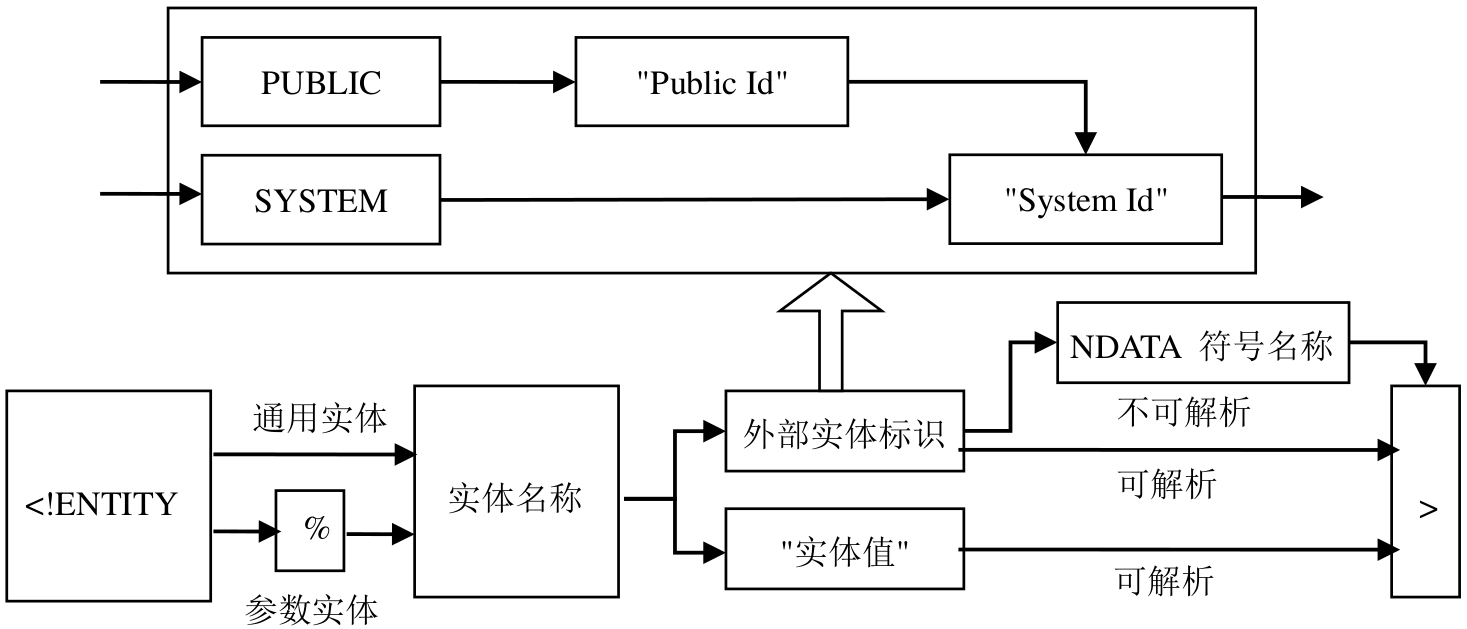
\includegraphics[width=0.9\textwidth]{figure/dtd-entity.png}
\end{figure}
\end{frame}



\subsubsection{3.5.2 内部可解析通用实体}
\begin{frame}[fragile]{3.5.2 内部可解析通用实体}
\begin{easylist} \easyitem    
& 语法形式:
\begin{lstlisting}[tabsize=8, basicstyle=\small\tt, language=XML, numbers=none]
<!ENTITY 实体名称 "实体值" >
\end{lstlisting}

& 例子
\begin{lstlisting}[tabsize=8, basicstyle=\small\tt, language=XML, numbers=none]
<?xml version = "1.0" encoding="utf-8"?>
<!DOCTYPE 数据 [
    <!ELEMENT 数据 (#PCDATA)>
    <!ENTITY 版权声明 "自由信息,由人民大学编写"> 
]>
<数据>&版权声明;</数据>
\end{lstlisting}
\end{easylist}
\end{frame}


\begin{frame}[fragile]{示例}
\begin{easylist} \easyitem    
& 可在实体的定义之中引用已定义实体
\begin{lstlisting}[tabsize=8, basicstyle=\small\tt, language=XML]
<!ENTITY 机构 "人民大学">
<!ENTITY 版权声明 "自由信息,由&机构;编写">
\end{lstlisting}

& 不可以相互引用,如:
\begin{lstlisting}[tabsize=8, basicstyle=\small\tt, language=XML]
<!ENTITY 机构 "人民大学, &版权声明;">
<!ENTITY 版权声明 "自由信息,由&机构;编写">
\end{lstlisting}

& 不能针对DTD的元素定义采用通用实体引用
\begin{lstlisting}[tabsize=8, basicstyle=\small\tt, language=XML]
<!ENTITY 教师基本信息 "(姓名, 性别, 出生年月, 研究方向)">
<!ELEMENT 教授 &教师基本信息;>
<!ELEMENT 副教授 &教师基本信息;>
<!ENTITY 讲师 &教师基本信息;>
\end{lstlisting}
\end{easylist}
\end{frame}


\subsubsection{3.5.3 外部可解析通用实体}
\begin{frame}[fragile]{3.5.3 外部可解析通用实体}
\begin{easylist} \easyitem    
& 语法形式:
\begin{lstlisting}[tabsize=8, basicstyle=\small\tt, language=XML, numbers=none]
<!ENTITY 实体名称 SYSTEM "系统标识符" >  
\end{lstlisting}
\begin{lstlisting}[tabsize=8, basicstyle=\small\tt, language=XML, numbers=none]
<!ENTITY 实体名称 PUBLIC FPI "公共标识符" >
\end{lstlisting}

& 例子
\begin{lstlisting}[tabsize=8, basicstyle=\small\tt, language=XML]
<?xml version = "1.0" encoding="utf-8"?>
<!DOCTYPE 数据 [
    <!ELEMENT 数据 (#PCDATA)>
    <!ENTITY 介绍数据 SYSTEM "intro.txt">    
]>
<数据>&介绍数据;</数据>
\end{lstlisting}
\end{easylist}
\end{frame}


\subsubsection{3.5.4 外部非解析通用实体}
\begin{frame}[fragile]{3.5.4 外部非解析通用实体}
\begin{easylist} \easyitem    
& 外部可解析通用实体可以把外部文件中的文本内容与DTD实体建立关联,并被XML解析器读取处理;
& 对于图片、音频、视频等二进制文件,如果在实体引用时仍然被解析,则会因特殊字符的存在而导致语法错误,为此,W3C引入了非解析实体(Unparsed Entity)概念
& 外部非解析通用实体的语法形式:
\begin{lstlisting}[tabsize=8, basicstyle=\small\tt, language=XML, numbers=none]
<!ENTITY 实体名称 SYSTEM "系统标识符" NDATA Type>
\end{lstlisting}
\begin{lstlisting}[tabsize=8, basicstyle=\small\tt, language=XML, numbers=none]
<!ENTITY 实体名称 PUBLIC FPI "公共标识符" NDATA Type>
\end{lstlisting}
&& Type代表实体类型,为已声明的NOTATION
\end{easylist}
\end{frame}


\begin{frame}[fragile]{外部非解析通用实体示例}
\begin{lstlisting}[tabsize=8, basicstyle=\small\tt, language=XML]
<?xml version = "1.0" encoding="utf-8"?>
<!DOCTYPE 数据 [
    <!ELEMENT 数据 (#PCDATA)>
    <!NOTATION JPG SYSTEM "image/jpeg">
    <!ENTITY 插图 SYSTEM "ruc_1.jpg" NDATA JPG>    
    <!ATTLIST 数据 插图 ENTITY #IMPLIED>    
]>
<数据 插图="插图">外部非解析通用实体示例</数据>
\end{lstlisting}
\end{frame}


\subsubsection{3.5.5 内部参数实体}
\begin{frame}[fragile]{3.5.5 内部参数实体}
\begin{easylist} \easyitem    
& 引入参数实体原因
&& 通用实体虽然可以在DTD中声明,但却无法在DTD中加以引用
& 参数实体一定是可解析实体
&& 内部参数实体
&& 外部参数实体
& 语法形式:
\begin{lstlisting}[tabsize=8, basicstyle=\small\tt, language=XML, numbers=none]
<!ENTITY % 实体名称 "实体值" >
\end{lstlisting}
&& 参数实体定义中的“\%”前后有空格
\end{easylist}
\end{frame}


\begin{frame}[fragile]{内部参数在内部子集中的声明和引用示例}
\begin{lstlisting}[tabsize=8, basicstyle=\small\tt, language=XML]
<?xml version = "1.0" encoding="utf-8"?>
<!DOCTYPE 教工信息 [
    <!ELEMENT 教工信息 ANY>
    <!ELEMENT 姓名 (#PCDATA)>
    <!ELEMENT 专业 (#PCDATA)>
    <!ENTITY % 教授信息 "<!ELEMENT 教授 (姓名, 专业)>">
    <!ENTITY % 讲师信息 "<!ELEMENT 讲师 (姓名, 专业)>">    
    %教授信息;
    %讲师信息;    
]>
<教工信息>
    <教授><姓名>钱钟书</姓名> <专业>国学</专业></教授>
</教工信息>
\end{lstlisting}

\begin{easylist} \easyitem    
& 思考:“教授”和“讲师”元素具备相同的声明内容,是否可以把这部分内容单独声明为参数实体,并在元素声明中加以引用?
\end{easylist}
\end{frame}


\begin{frame}[fragile]{内部参数在内部子集中的声明和引用示例}
\begin{lstlisting}[tabsize=8, basicstyle=\small\tt, language=XML]
<?xml version = "1.0" encoding="utf-8"?>
<!DOCTYPE 教工信息 [
    <!ELEMENT 教工信息 ANY>
    <!ELEMENT 姓名 (#PCDATA)>
    <!ELEMENT 专业 (#PCDATA)>
    <!ENTITY % 教师基本信息 "(姓名, 专业)">
    <!ELEMENT 教授 %教师基本信息;>
    <!ELEMENT 讲师 %教师基本信息;>
]>
<教工信息>
    <教授><姓名>钱钟书</姓名> <专业>国学</专业></教授>
</教工信息>
\end{lstlisting}

\begin{easylist} \easyitem    
& {\color{red}禁止在DTD内部子集中使用这种方式}
\end{easylist}
\end{frame}


\begin{frame}[fragile]{内部参数实体在外部子集中的声明和引用示例}


\begin{easylist} \easyitem    
& DTD文档:3-18.dtd
\begin{lstlisting}[tabsize=8, basicstyle=\small\tt, language=XML]
<?xml version="1.0" encoding="UTF-8"?>
<!ENTITY % 教师基本信息 "(姓名, 专业)">
<!ELEMENT 教授 %教师基本信息;>
<!ELEMENT 讲师 %教师基本信息;>
\end{lstlisting}

& XML文档:3-18.xml
\begin{lstlisting}[tabsize=8, basicstyle=\small\tt, language=XML]
<?xml version = "1.0" encoding="utf-8"?>
<!DOCTYPE 教工信息 SYSTEM "3-18.dtd"[
    <!ELEMENT 教工信息 ANY>
    <!ELEMENT 姓名 (#PCDATA)>
    <!ELEMENT 专业 (#PCDATA)>
    <!ENTITY % 教师基本信息 "(专业,姓名)">
]>
<教工信息>
    <教授>
        <专业>国学</专业><姓名>钱钟书</姓名>
    </教授>
</教工信息>
\end{lstlisting}
\end{easylist}
\end{frame}



\subsubsection{3.5.6 外部参数实体}
\begin{frame}[fragile]{3.5.6 外部参数实体}
\begin{easylist} \easyitem    
& 外部参数实体用于包含来自外部资源的声明
&& 参数实体总是可解析的,一个到外部参数实体的引用(\%参数实体名称;)将被替换为解析后的内容
& 外部参数实体的语法
\begin{lstlisting}[tabsize=8, basicstyle=\small\tt, language=XML, numbers=none]
<!ENTITY % 实体名称 SYSTEM "系统标识符"> 
<!ENTITY % 实体名称 PUBLIC FPI "公共标识符">
\end{lstlisting}

& 作用
&& 可以把多个较小的DTD文件组成一个更大的DTD声明,或者把一个大的DTD分解为小的、更便于管理的模块,方便理解和重复使用
\end{easylist}
\end{frame}


\begin{frame}[fragile, allowframebreaks]{外部参数实体示例}
\begin{easylist} \easyitem    
& 外部DTD文件“3-20\_1.dtd”
\begin{lstlisting}[tabsize=8, basicstyle=\small\tt, language=XML]
<!ELEMENT 外观 (颜色, 体积)>
<!ELEMENT 颜色 (#PCDATA)>
<!ELEMENT 体积 (#PCDATA)>
\end{lstlisting}

& 外部DTD文件“3-20\_2.dtd”
\begin{lstlisting}[tabsize=8, basicstyle=\small\tt, language=XML]
<!ELEMENT 联系方式 (客服电话, 网址)>
<!ELEMENT 客服电话 (#PCDATA)>
<!ELEMENT 网址 (#PCDATA)>
\end{lstlisting}
\newpage

& XML文件“3-20.xml”
\begin{lstlisting}[tabsize=8, basicstyle=\small\tt, language=XML]
<?xml version = "1.0" encoding="utf-8"?>
<!DOCTYPE 家具 [
    <!ELEMENT 家具 (名称, 外观, 联系方式)>
    <!ELEMENT 名称 (#PCDATA)>
    <!ENTITY % 外观 SYSTEM "3-20_1.dtd">
    <!ENTITY % 联系方式 SYSTEM "3-20_2.dtd">
    %外观;
    %联系方式;
]>
<家具>    
    <名称>布艺沙发</名称>
    <外观>
        <颜色>白色</颜色>
        <体积>3.4*2.55</体积>
    </外观>
    <联系方式>
        <客服电话>400-800-1234</客服电话>
        <网址>http://www.example.com/</网址>
    </联系方式>
</家具>
\end{lstlisting}
\end{easylist}
\end{frame}


\subsection{3.6 DTD NOTATION}
\begin{frame}[fragile]{3.6 DTD NOTATION}
\begin{easylist} \easyitem    
& 用于识别非解析实体格式的名字
& 用于DTD引用外部文件数据的情况
&& 图像、声音等二进制文件可能包含各种XML无法处理的特殊符号,此时需要借助于外部的应用程序进行处理,这类情况的解释描述可以通过NOTATION实现

& DTD NOTATION的语法格式
\begin{lstlisting}[tabsize=8, basicstyle=\small\tt, language=XML, numbers=none]
<!NOTATION 名称 SYSTEM "系统标识">
<!NOTATION名称 PUBLIC "公共标识" >
\end{lstlisting}

& 例子
\begin{lstlisting}[tabsize=8, basicstyle=\small\tt, language=XML]
<!NOTATION gif SYSTEM "image/gif">
\end{lstlisting}
\end{easylist}
\end{frame}


\subsection{3.7 DTD的包含与忽略}
\begin{frame}[fragile]{3.7 DTD的包含与忽略}
\begin{easylist} \easyitem    
& INCLUDE
& IGNORE
& 语法格式
\begin{lstlisting}[tabsize=8, basicstyle=\small\tt, language=XML]
<!INCLUDE [ 
    此处为DTD声明内容
]]> 
<!INGORE [ 
    此处为DTD声明内容
]]> 
\end{lstlisting}

\end{easylist}
\end{frame}

\begin{frame}[fragile]{INCLUDE与IGNORE示例}
\begin{lstlisting}[tabsize=8, basicstyle=\small\tt, language=XML]
<!-- Tables Module .............. -->
<!ENTITY % xhtml-table.module "INCLUDE" >
<![%xhtml-table.module;[
<!ENTITY % xhtml-table.mod
            PUBLIC "-//W3C//ELEMENTS XHTML Tables 1.0//EN"
            "http://www.w3.org/MarkUp/DTD/xhtml-table-1.mod" >
%xhtml-table.mod;]]>
\end{lstlisting}
\begin{easylist} \easyitem
& 行2和行3展示了INCLUDE的使用方式,
& 如不包含该段声明,只需要把第2行中的参数实体值更改为IGNORE即可
& 行4和行5则展示了外部参数实体的作用。
\end{easylist}
\end{frame}


\begin{frame}
\begin{center}
    \Huge END
\end{center}
\begin{figure}
    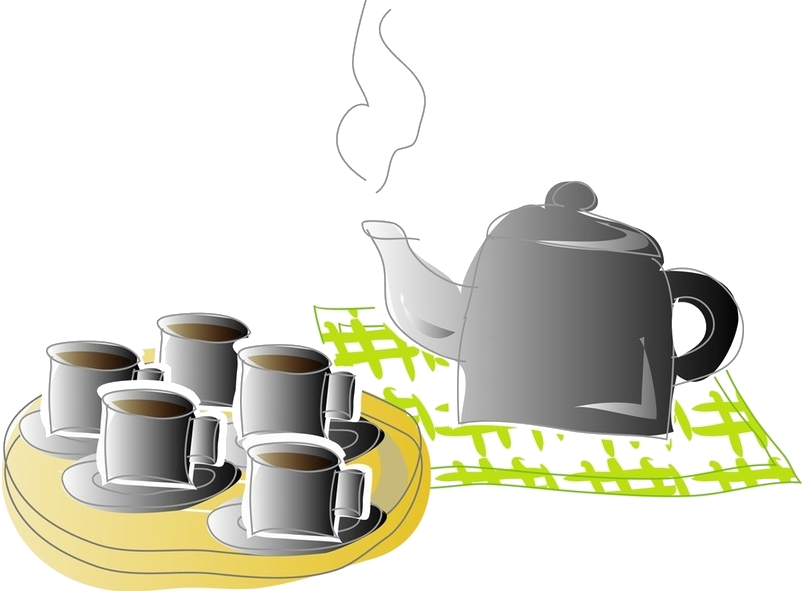
\includegraphics[width=0.75\textwidth]{figure/relax.png}
\end{figure}
\end{frame}